\documentclass[border=8pt]{standalone}
% shared preamble for lecture topic figures (compile from beamer/ with xelatex)
\usepackage{tikz}
\usepackage{fontspec}
\usepackage{amsmath}
\usetikzlibrary{arrows.meta,positioning,calc,backgrounds,fit,decorations.pathmorphing}
\setsansfont{SpaceGrotesk}[Path=fonts/,Extension=.ttf,UprightFont=*-400,BoldFont=*-700,FontFace={md}{n}{*-500}]
\renewcommand{\familydefault}{\sfdefault}
\definecolor{navy}{HTML}{182B49}
\definecolor{gold}{HTML}{C8881E}
\definecolor{teal}{HTML}{1F6F86}
\definecolor{green}{HTML}{157E6B}
\definecolor{stone}{HTML}{F7F6F2}
\definecolor{ink}{HTML}{182B49}
\tikzset{
  card/.style={fill=white, rounded corners=4pt, draw=navy!15, line width=0.5pt},
  flow/.style={-{Stealth[length=4pt]}, navy, line width=0.9pt},
  lab/.style={text=navy, font=\sffamily\fontsize{8}{9}\selectfont},
  toplab/.style={text=navy!65, font=\sffamily\fontsize{8.5}{10}\selectfont},
}

\begin{document}
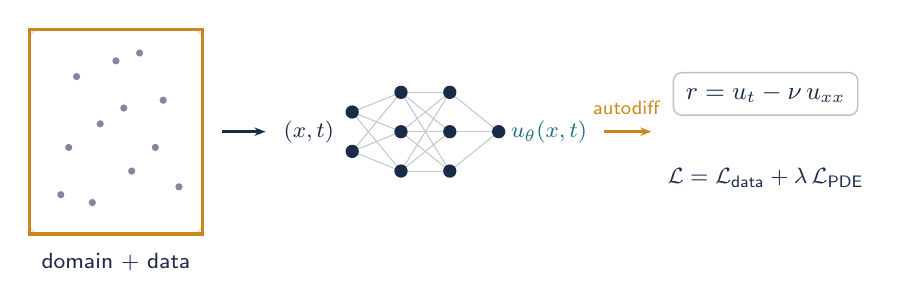
\begin{tikzpicture}
  % domain with collocation points
  \path[card] (0,0) rectangle (2.2,2.6);
  \foreach \px/\py in {0.4/0.5,0.9/1.4,0.6/2.0,1.3/0.8,1.7/1.7,1.1/2.2,0.5/1.1,1.9/0.6,1.4/2.3,0.8/0.4,1.6/1.1,1.2/1.6}{
    \fill[navy!55] (\px,\py) circle (1.3pt);
  }
  \draw[gold, line width=1.2pt] (0,0) rectangle (2.2,2.6);
  \node[lab] at (1.1,-0.35) {domain $+$ data};

  \draw[flow] (2.45,1.3) -- (3.0,1.3);
  \node[navy, font=\sffamily\fontsize{8.5}{10}\selectfont] at (3.55,1.3) {$(x,t)$};

  % small MLP
  \begin{scope}[shift={(4.1,0)}]
    \foreach \l/\n/\xs in {0/2/0, 1/3/1, 2/3/2, 3/1/3}{
      \foreach \k in {1,...,\n}{
        \coordinate (n\l-\k) at (\xs*0.62,{1.3+(\k-(\n+1)/2)*0.5});
      }
    }
    \foreach \a in {1,2}{\foreach \b in {1,2,3}{\draw[navy!25,line width=0.4pt] (n0-\a)--(n1-\b);}}
    \foreach \a in {1,2,3}{\foreach \b in {1,2,3}{\draw[navy!25,line width=0.4pt] (n1-\a)--(n2-\b);}}
    \foreach \a in {1,2,3}{\draw[navy!25,line width=0.4pt] (n2-\a)--(n3-1);}
    \foreach \l/\n in {0/2,1/3,2/3,3/1}{\foreach \k in {1,...,\n}{\fill[navy] (n\l-\k) circle (2.4pt);}}
  \end{scope}

  \node[teal, font=\sffamily\bfseries\fontsize{8.5}{10}\selectfont] (u) at (6.6,1.3) {$u_\theta(x,t)$};
  \draw[flow] (5.95,1.3) -- (6.05,1.3);

  % autodiff -> residual
  \draw[flow, gold] (7.3,1.3) -- (7.9,1.3);
  \node[text=gold, font=\sffamily\fontsize{7}{8}\selectfont] at (7.58,1.6) {autodiff};
  \node[draw=navy!30, fill=white, rounded corners=3pt, text=navy, inner sep=4.5pt,
        line width=0.5pt, font=\sffamily\fontsize{9}{11}\selectfont] (res) at (9.35,1.78)
        {$r = u_t-\nu\,u_{xx}$};
  \node[text=navy, font=\sffamily\fontsize{8.5}{12}\selectfont] at (9.35,0.72)
    {$\mathcal{L}=\mathcal{L}_{\text{data}}+\lambda\,\mathcal{L}_{\text{PDE}}$};
\end{tikzpicture}
\end{document}
